% TU Delft beamer template
% Author: Erwin Walraven (initial version was created by Maarten Abbink)
% Delft Universiy of Technology

\documentclass{beamer}
\usepackage[english]{babel}
\usepackage{calc}
\usepackage[absolute,overlay]{textpos}
\usepackage{graphicx}
\usepackage{subfig}
\usepackage{amsmath}
\usepackage{amsfonts}
\usepackage{amsthm}
\usepackage{mathtools}
\usepackage{comment}
\usepackage{MnSymbol,wasysym}
\usepackage{url}
\usepackage{fancyhdr}
\usepackage{subfig}
\usepackage[export]{adjustbox}
\DeclarePairedDelimiter\floor{\lfloor}{\rfloor}

\setbeamertemplate{navigation symbols}{} % remove navigation symbols
\mode<presentation>{\usetheme{tud}}

% BIB SETTINGS
\usepackage[backend=bibtex,firstinits=true,maxnames=30,maxcitenames=20,url=false,style=authoryear]{biblatex}
\bibliography{bibfile}
\setlength\bibitemsep{0.3cm} % space between entries in the reference list
\renewcommand{\bibfont}{\normalfont\scriptsize}
\setbeamerfont{footnote}{size=\tiny}
\renewcommand{\cite}[1]{\footnote<.->[frame]{\fullcite{#1}}}

\title[]{QAOA performance on MaxCut \\ for various graphs using Rigetti's QVM}
\institute[]{Technische Universiteit Delft, Nederland}
\author{Joost Bus \\ \tiny{j.c.p.bus@student.tudelft.nl}}
\date{\today}

\begin{document}
{
\setbeamertemplate{footline}{\usebeamertemplate*{minimal footline}}
\frame{\titlepage}
}
{\setbeamertemplate{footline}{\usebeamertemplate*{minimal footline}}}

% Overview
\begin{frame}{Overview}
\tableofcontents
\end{frame}

% Disclaimers
\begin{frame}{Disclaimers}
	\begin{itemize}
		\item I ran these experiments using the pyQuil QVM; these are all simulated
		\item These simulations were run \textbf{without noise simulation}
		\item The algorithm works on arbitrary graphs and for various integers $p$. Therefore it disregards possible restrictions on the topology of the QPU
		\item The angle optimisation is done using VQE, which is also simulated without noise
		\item For each graph I used 10000 samples. However, the angles are also chosen stochastically (using VQE) therefore the algorithm does not produce the same result with the same inputs.
		\item The presentation of results is not optimal, in the future I would like to present all possible bitstring (to show contrast / interference) and moreover group the bitstring together with the same cost.
	\end{itemize}
\end{frame}

% Butterfly
\section{Graphs}
\subsection{Butterfly}
\begin{frame}{Butterfly}
	\begin{figure}
		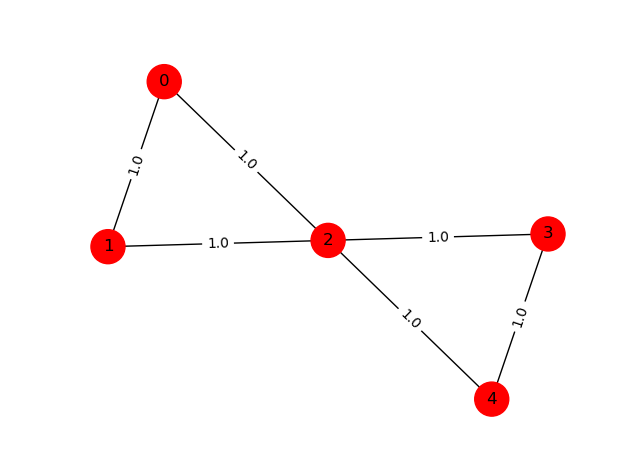
\includegraphics[scale=0.6]{figures/butterfly-graph.png}
		\caption*{Observe that every $2-3$ cut is optimal, as is the cut $00100 \hateq 11011$}
	\end{figure}
\end{frame}

\begin{frame}{Butterfly, $p = 1$}
\begin{figure}
	\centering
	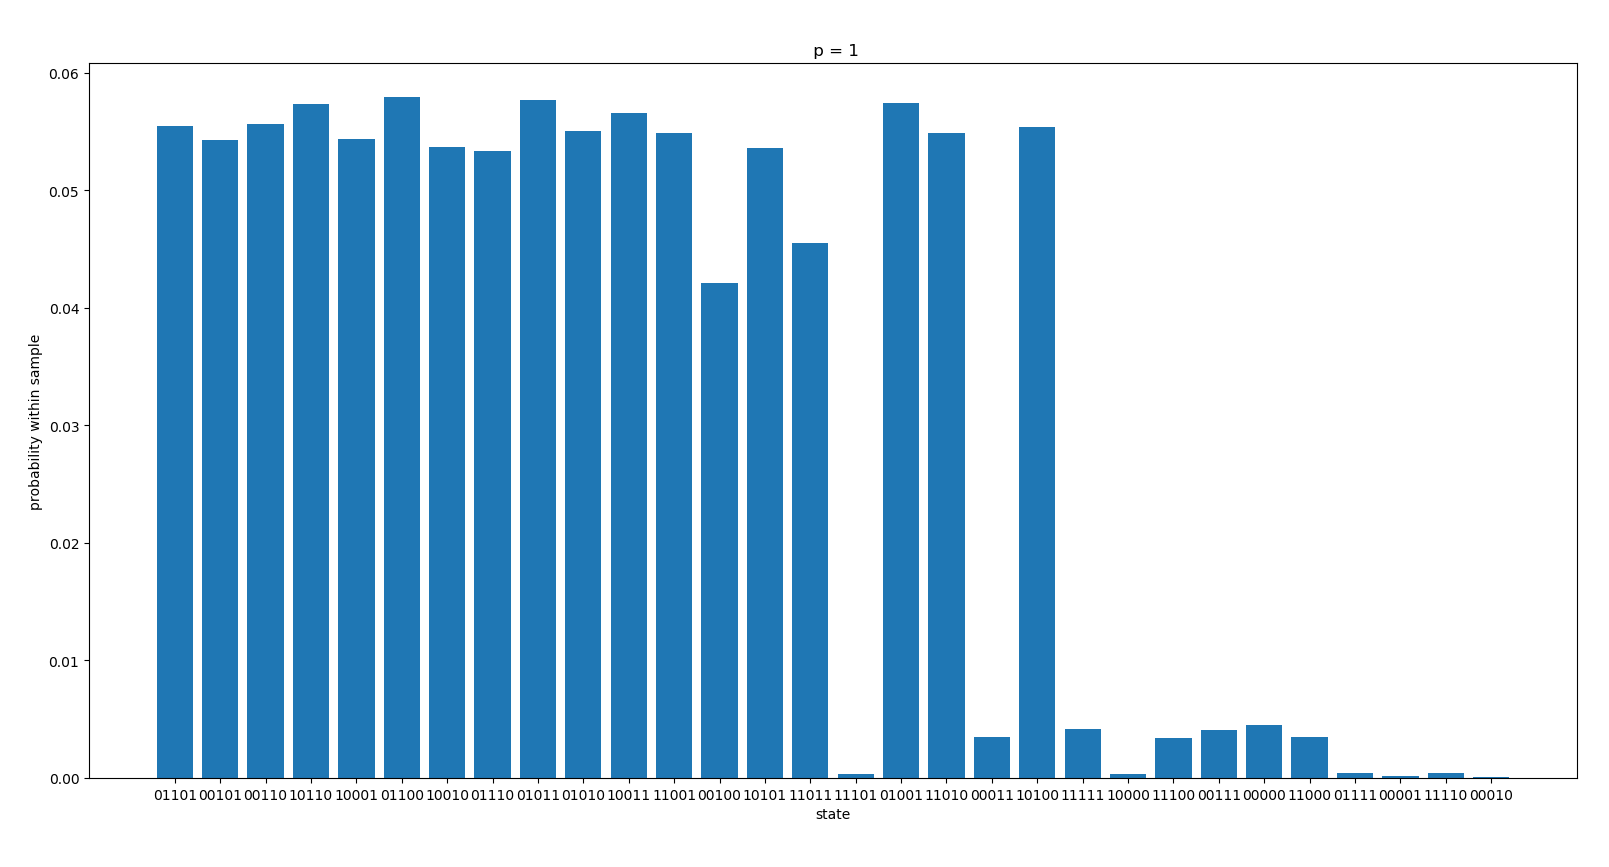
\includegraphics[scale=0.3,left]{figures/butterfly-p1.png}
\end{figure}
\end{frame}

\begin{frame}{Butterfly, $p = 2$}
\begin{figure}
	\centering
	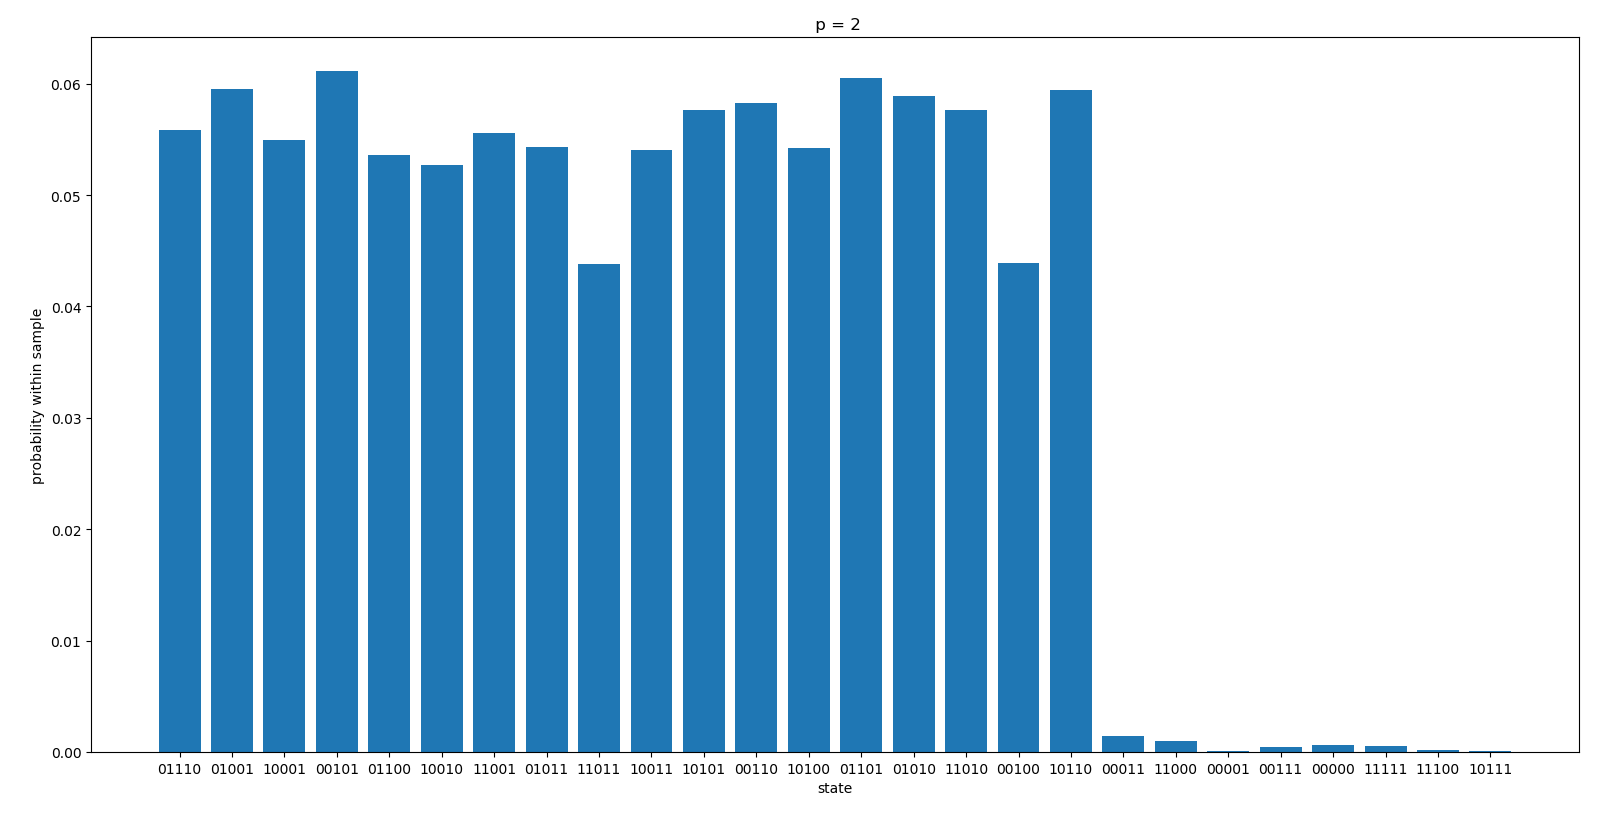
\includegraphics[scale=0.3,left]{figures/butterfly-p2.png}
\end{figure}
\end{frame}

\begin{frame}{Butterfly, $p = 3$}
\begin{figure}
	\centering
	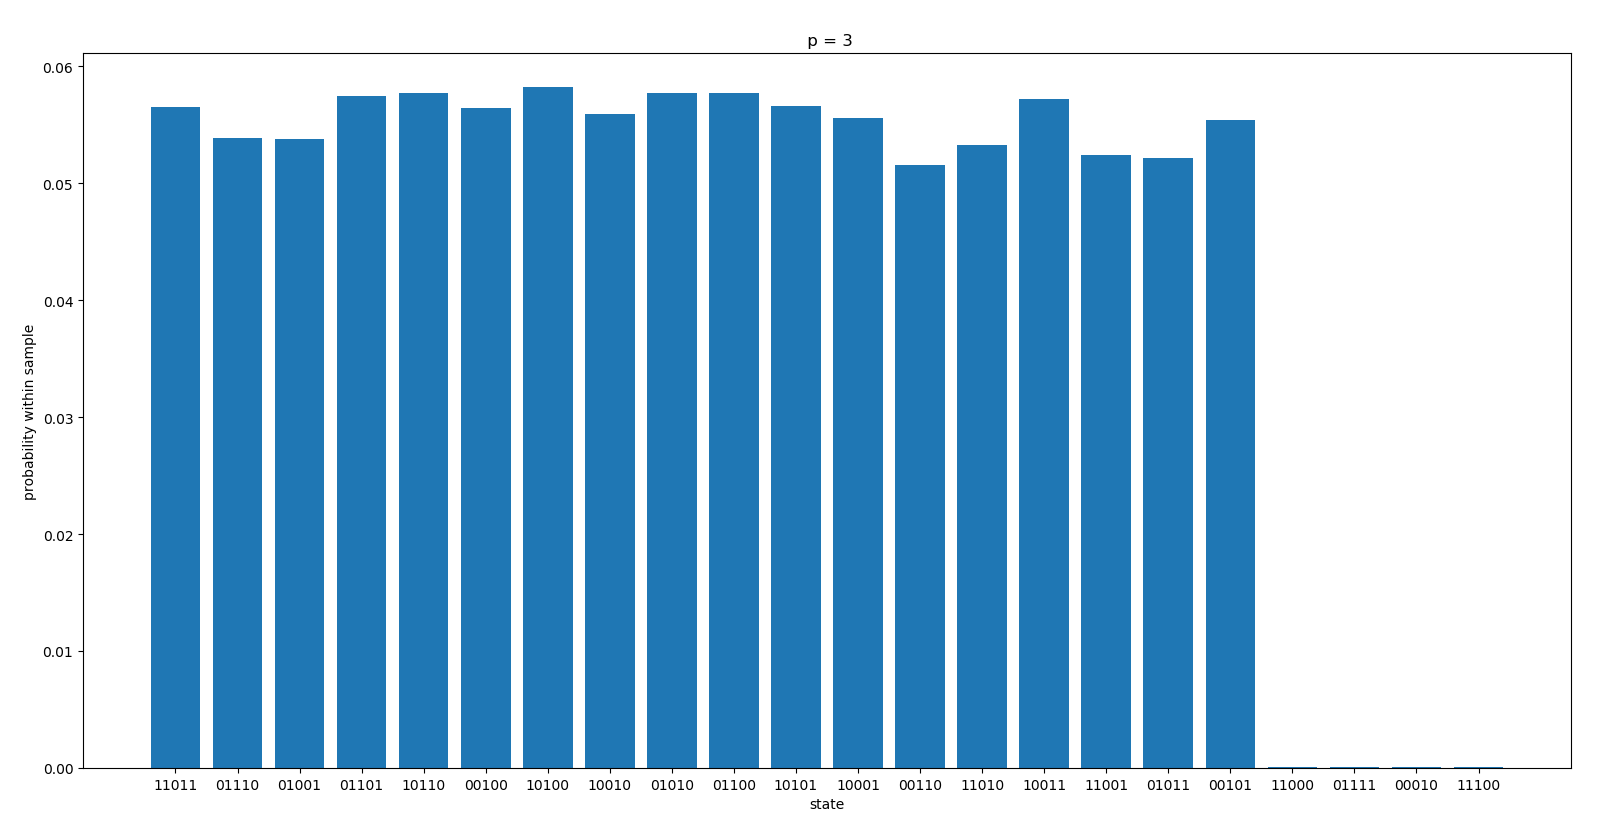
\includegraphics[scale=0.3,left]{figures/butterfly-p3.png}
\end{figure}
\end{frame}

\begin{frame}{Butterfly, pushing it to p = 10}
\begin{figure}
	\centering
	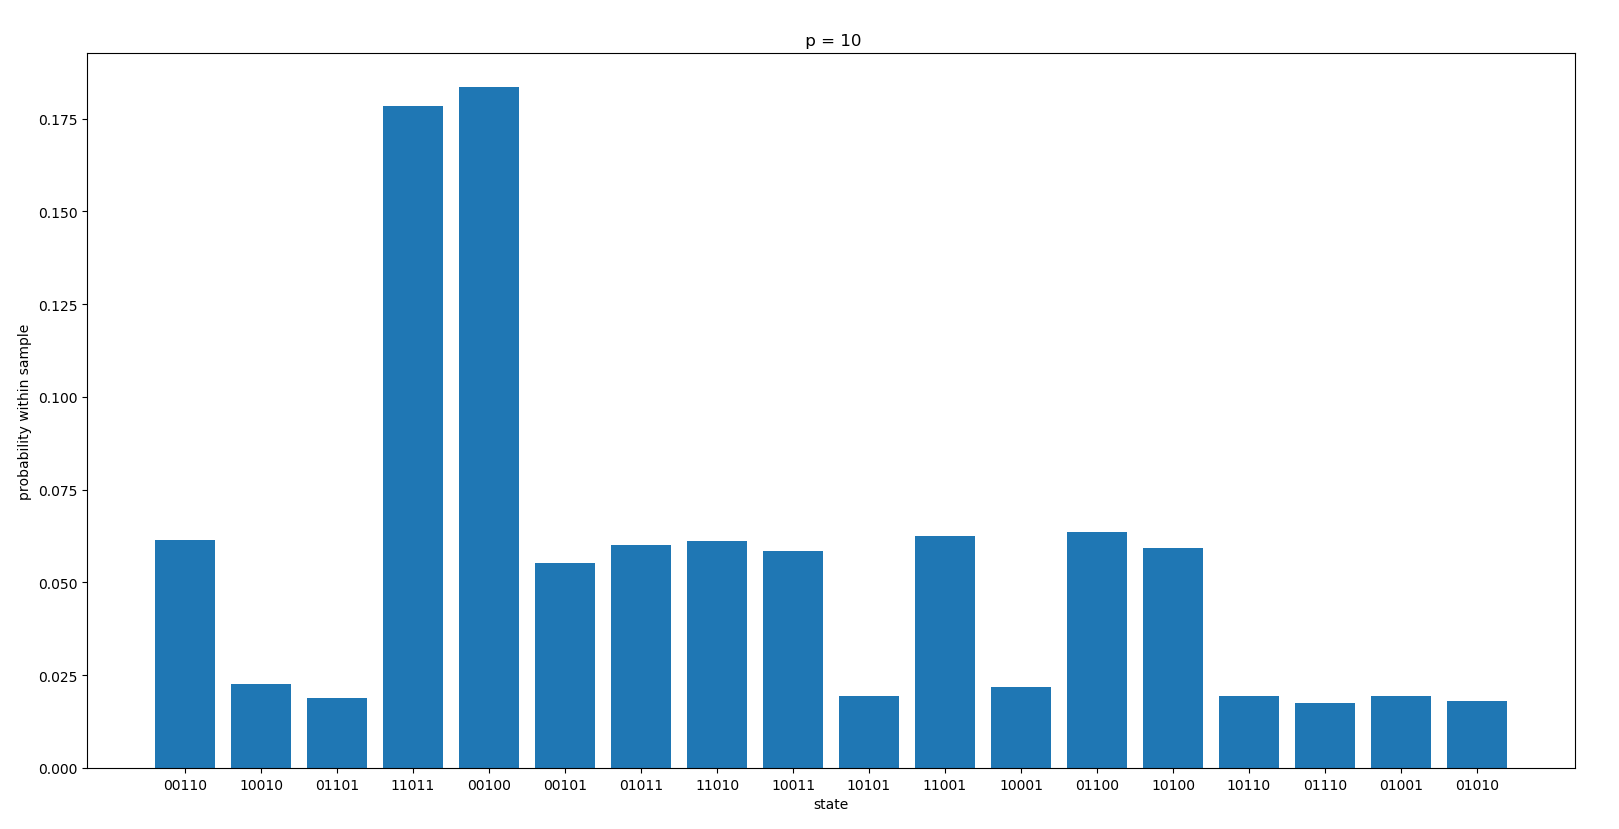
\includegraphics[scale=0.3,left]{figures/butterfly-p10.png}
\end{figure}
\end{frame}

% Diamond
\subsection{Diamond}
\begin{frame}{Diamond}
\begin{figure}
	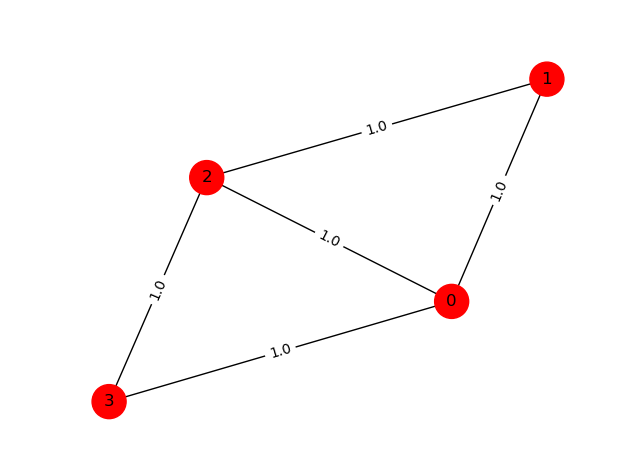
\includegraphics[scale=0.6]{figures/diamond-graph.png}
\end{figure}
\end{frame}

\begin{frame}{Diamond}
\begin{figure}
	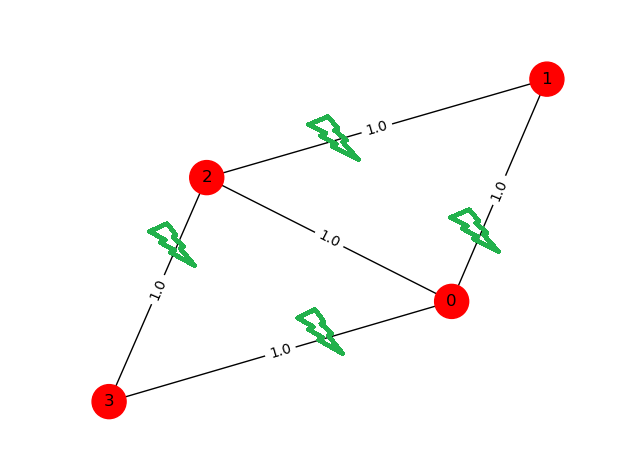
\includegraphics[scale=0.6]{figures/diamond-cut.png}
	\caption*{Observe that there are two optimal cuts: $1010$ and $0101$}
\end{figure}
\end{frame}

\begin{frame}{Diamond, $p = 1$}
\begin{figure}
	\centering
	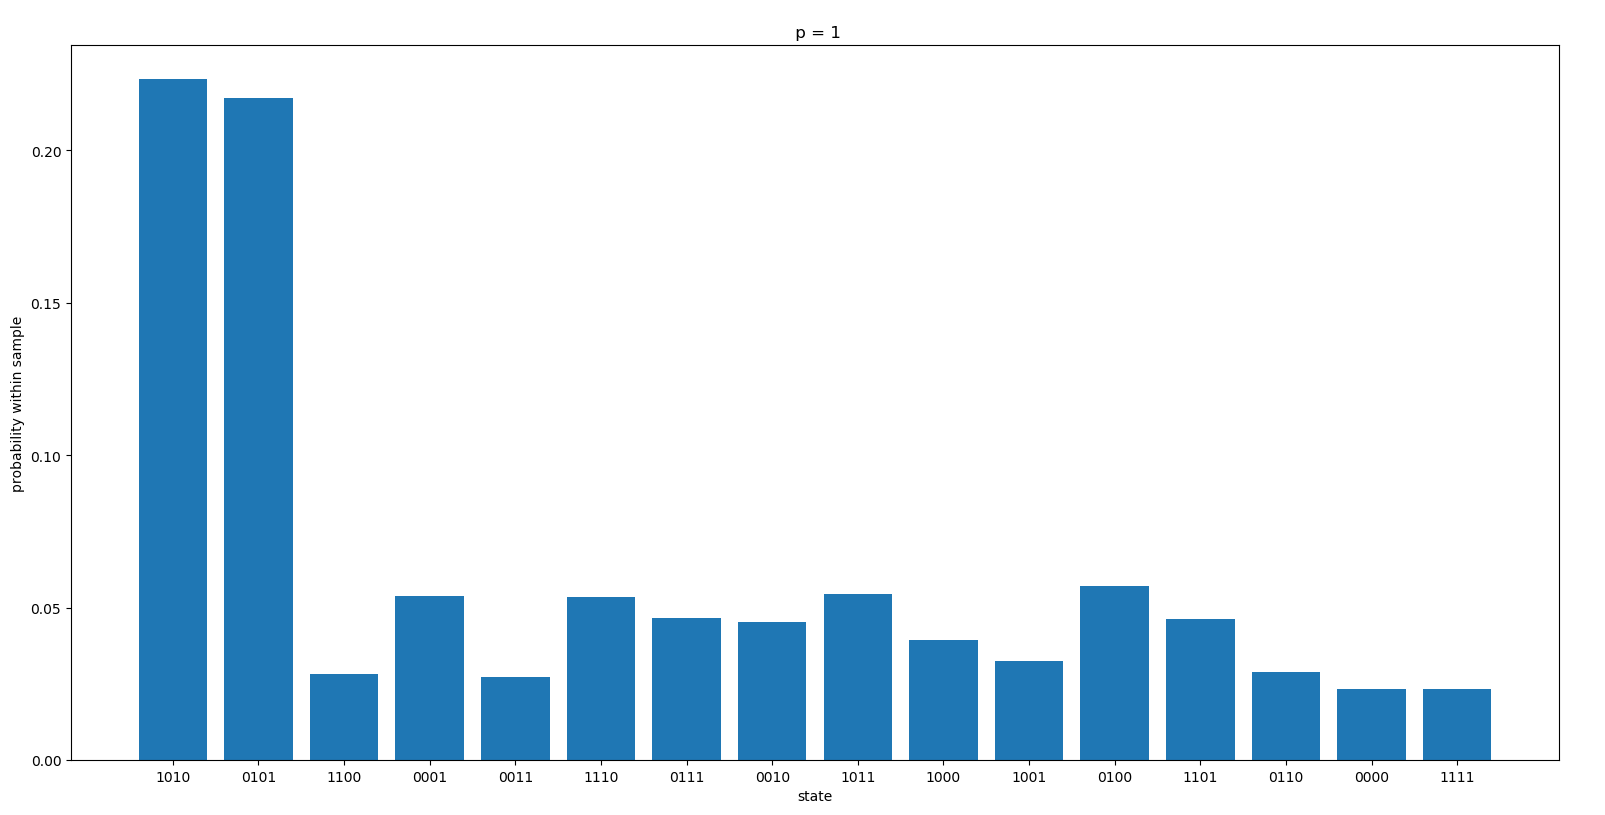
\includegraphics[scale=0.3,left]{figures/diamond-p1.png}
\end{figure}
\end{frame}

\begin{frame}{Diamond, $p = 2$}
\begin{figure}
\centering
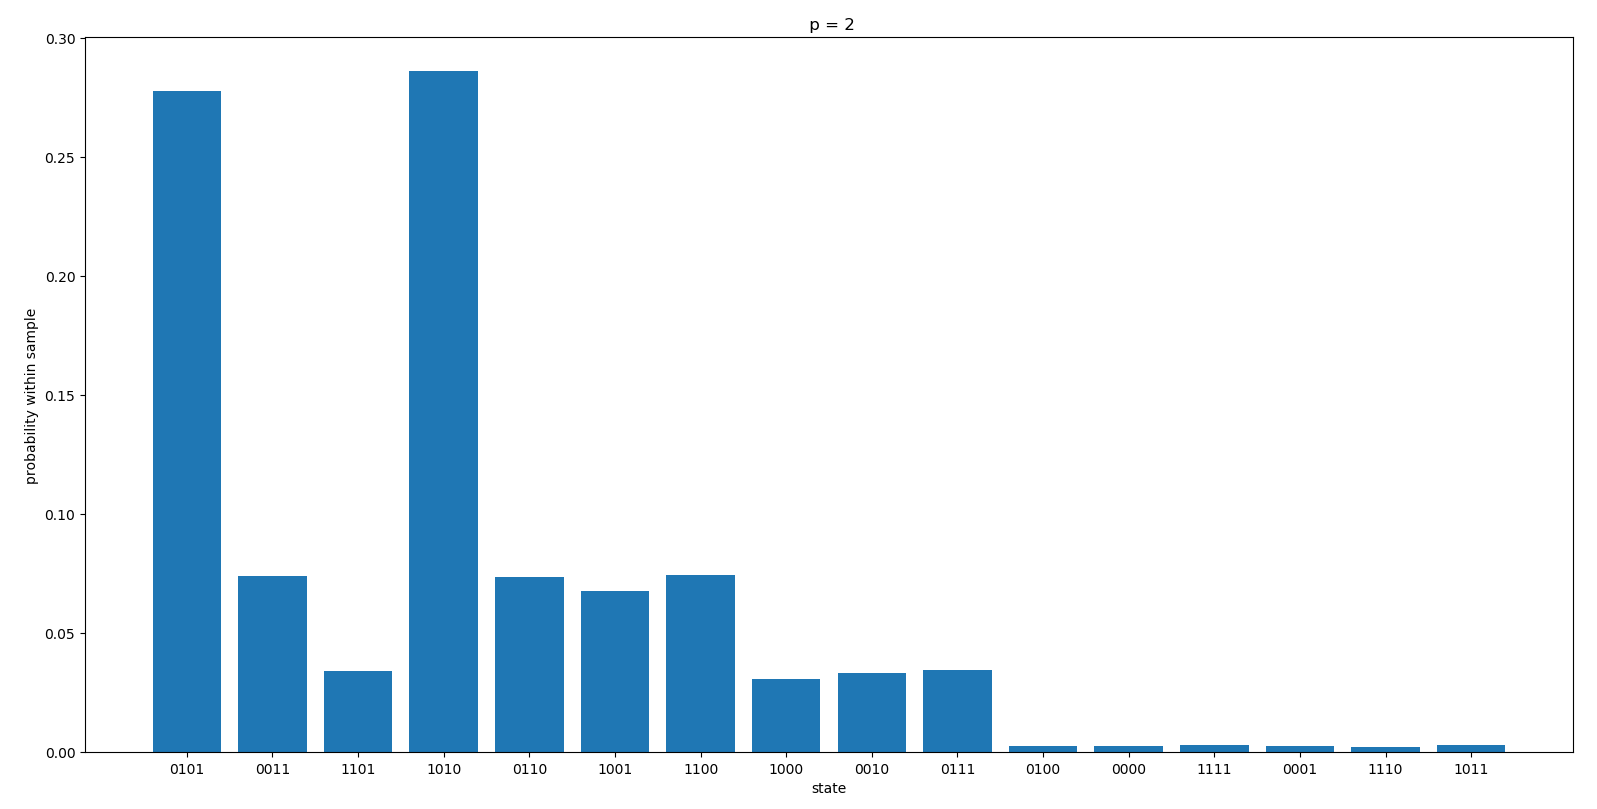
\includegraphics[scale=0.3,left]{figures/diamond-p2.png}
\end{figure}
\end{frame}

\begin{frame}{Diamond, $p = 3$}
\begin{figure}
\centering
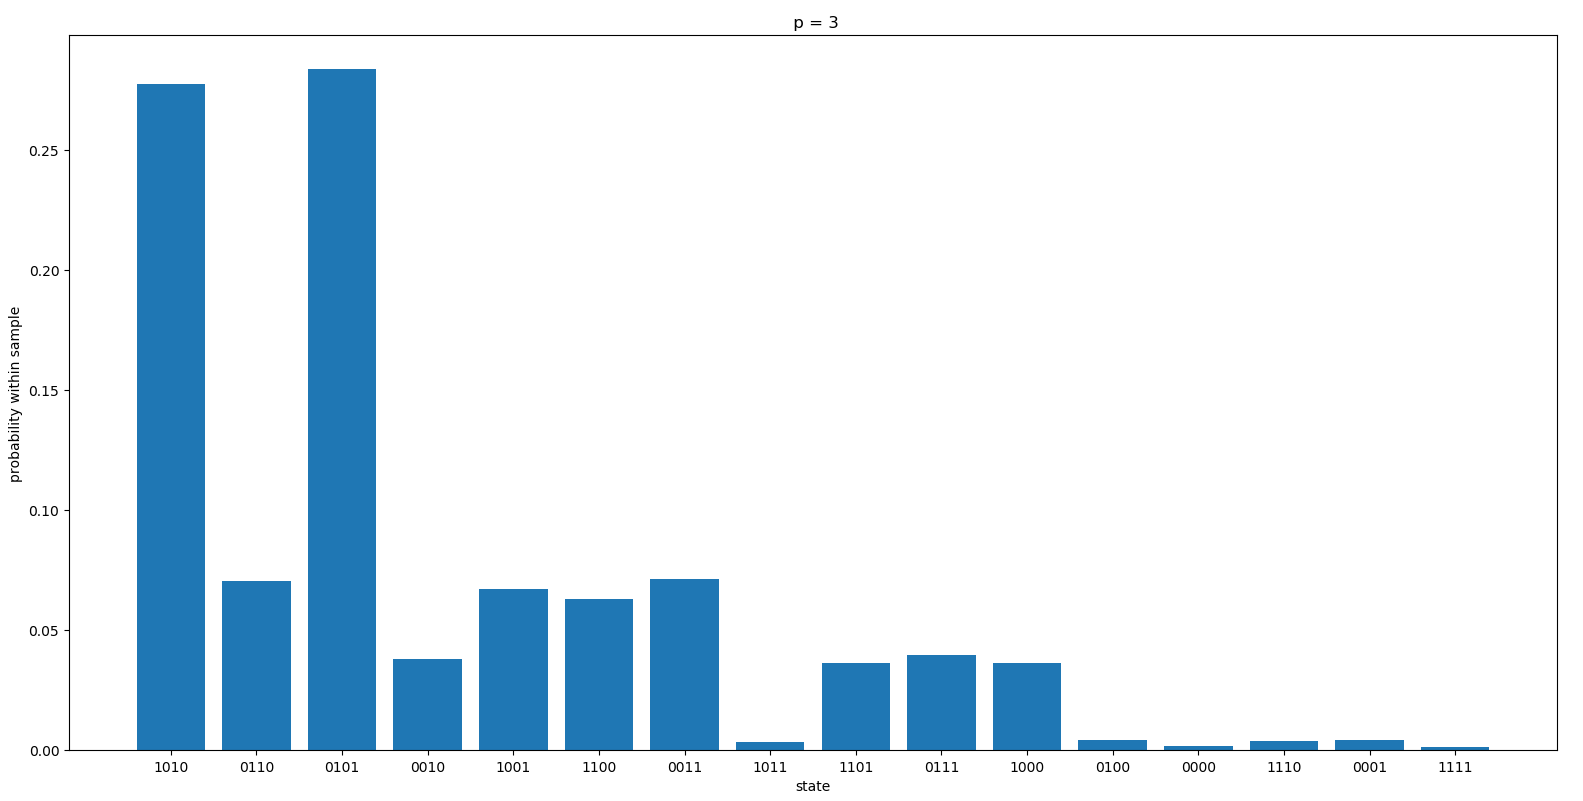
\includegraphics[scale=0.3,left]{figures/diamond-p3.png}
\end{figure}
\end{frame}

\begin{frame}{Diamond, $p = 4$}
\begin{figure}
	\centering
	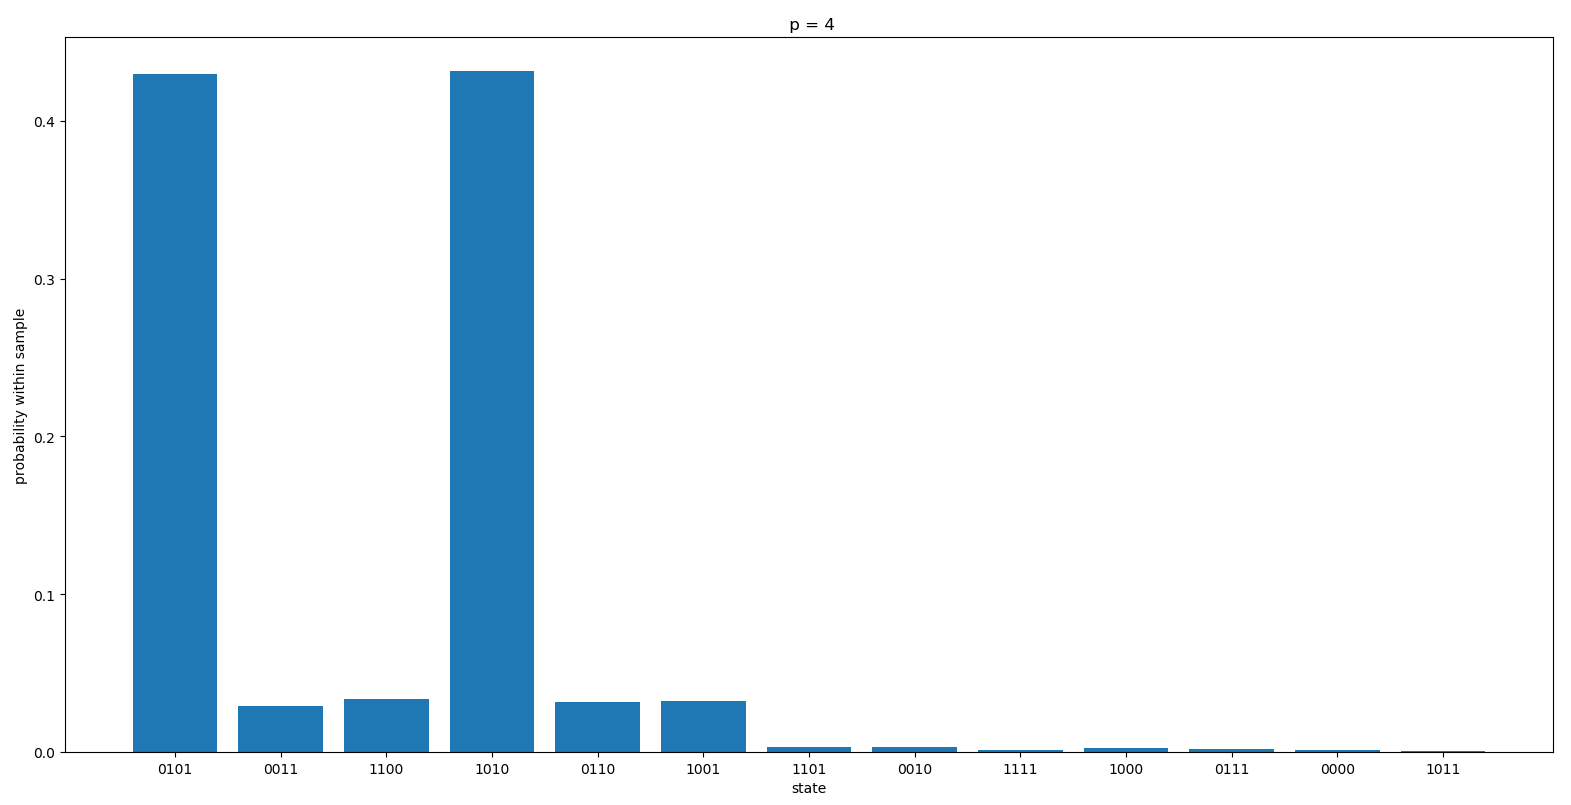
\includegraphics[scale=0.3,left]{figures/diamond-p4.png}
\end{figure}
\end{frame}

\begin{frame}{Diamond, $p = 5$}
\begin{figure}
	\centering
	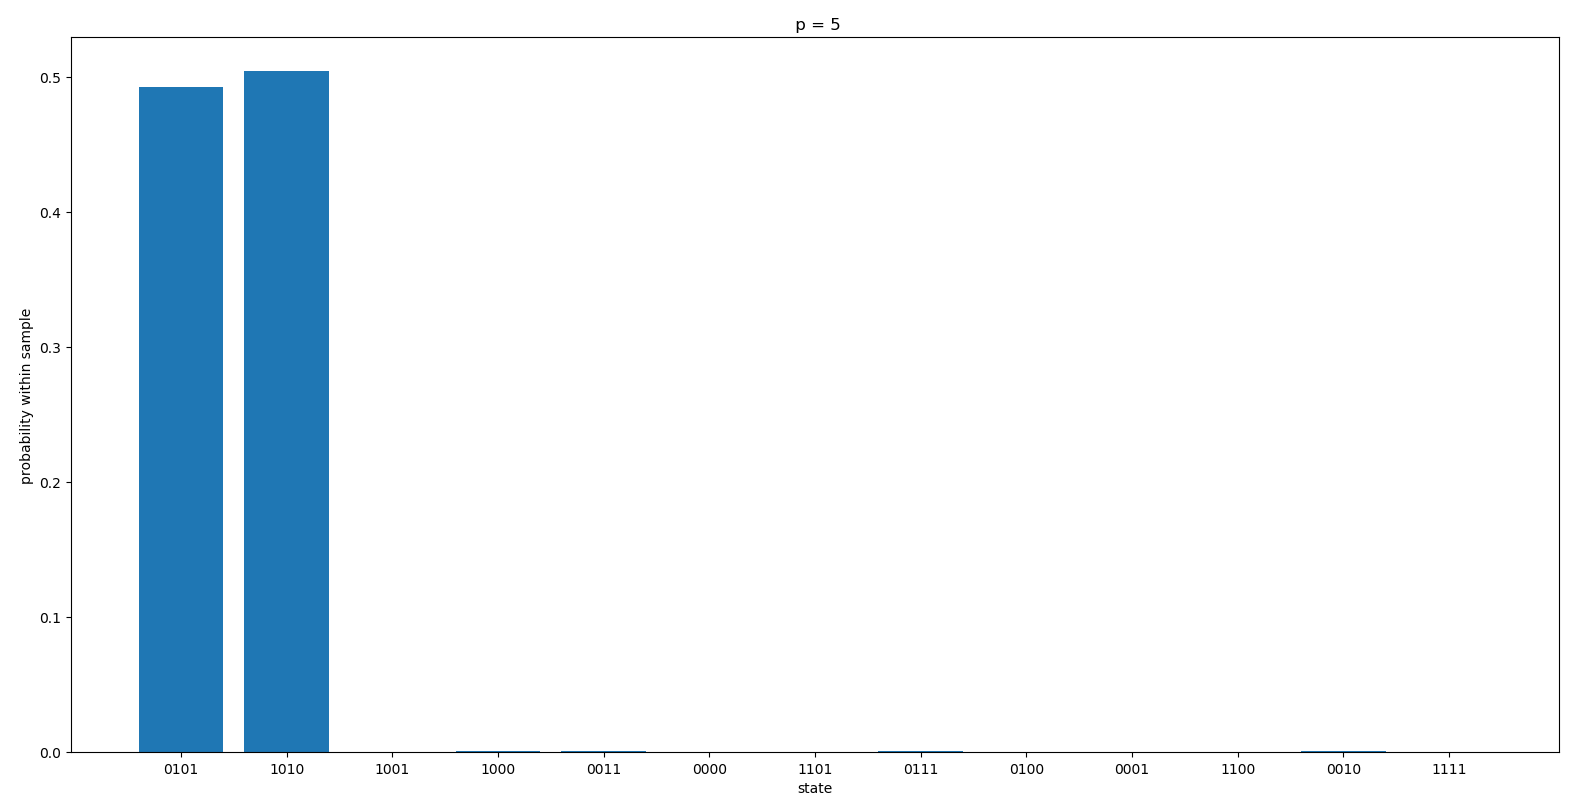
\includegraphics[scale=0.3,left]{figures/diamond-p5.png}
\end{figure}
\end{frame}

\subsection{Cycle graphs}
\begin{frame}{Cyclic graphs (connected 2-regular graphs)}
\begin{figure}
	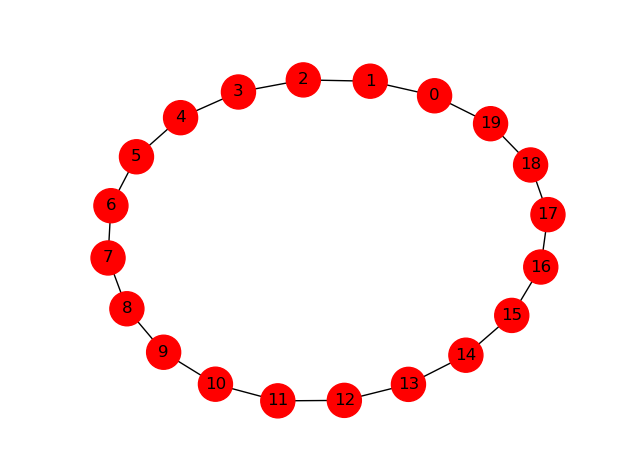
\includegraphics[scale=0.6]{figures/cycle20-graph.png}
	\caption*{The optimal cut for these graphs is $\floor{\frac{N}{2}}$, i.e. just alternating $1$ and $0$ (for odd degree there has to be one neighbour pair in the same set)}
\end{figure}
	
\end{frame}

\begin{frame}{Cycle-20, $p = 1$}
On a graph with 20 nodes it takes quite a while before the VQE (simulator) determined the optimal angles... ($\sim$3 min) \\~\\
The histogram is not very insightful as it is very wide. However, we did find the right solution, namely the alternating one
\begin{figure}
	\centering
	\begin{figure}
		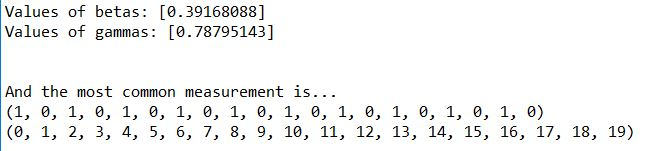
\includegraphics[scale=0.7]{figures/cycle20-p1.JPG}
	\end{figure}
	
\end{figure}
\end{frame}

\subsection{3-regular graphs}
% 3-regular, 4 nodes
\begin{frame}{3-regular graphs - 4 nodes}
\begin{figure}
	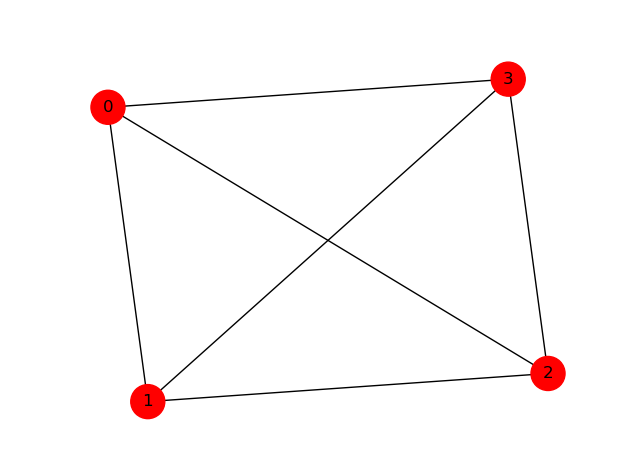
\includegraphics[scale=0.6]{figures/regular(3,4)-graph.png}
	\caption*{Observe that every $2-2$ cut is optimal, therefore there are ${4 \choose 2} = 6$ optimal cuts with value 4}
\end{figure}
\end{frame}

\begin{frame}{(3,4)-regular, $p = 1$}
\begin{figure}
\centering
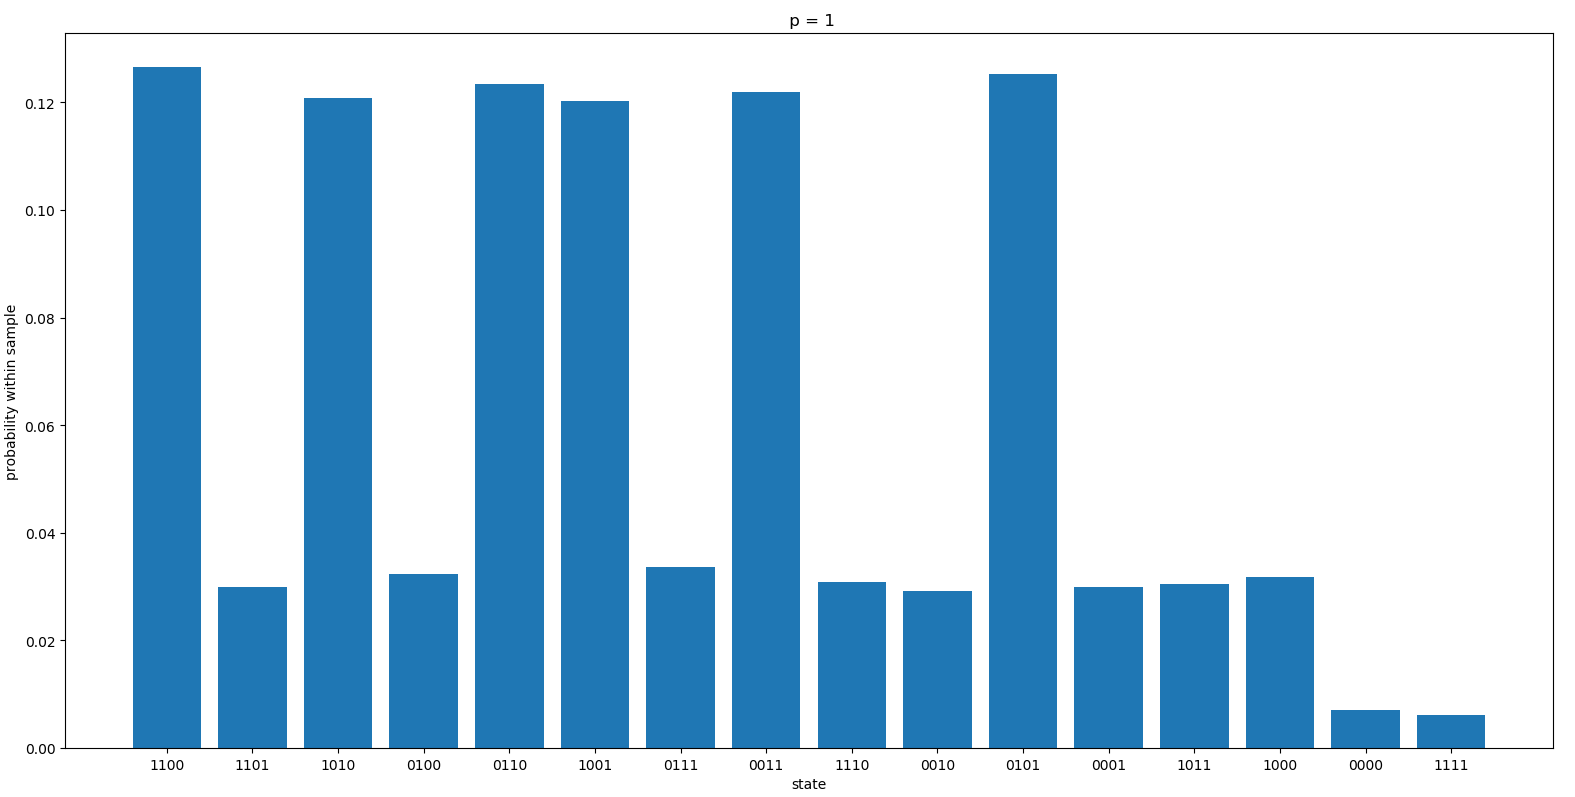
\includegraphics[scale=0.3,left]{figures/regular(3,4)-p1.png}
\end{figure}
\end{frame}

\begin{frame}{(3,4)-regular, $p = 2$}
\begin{figure}
\centering
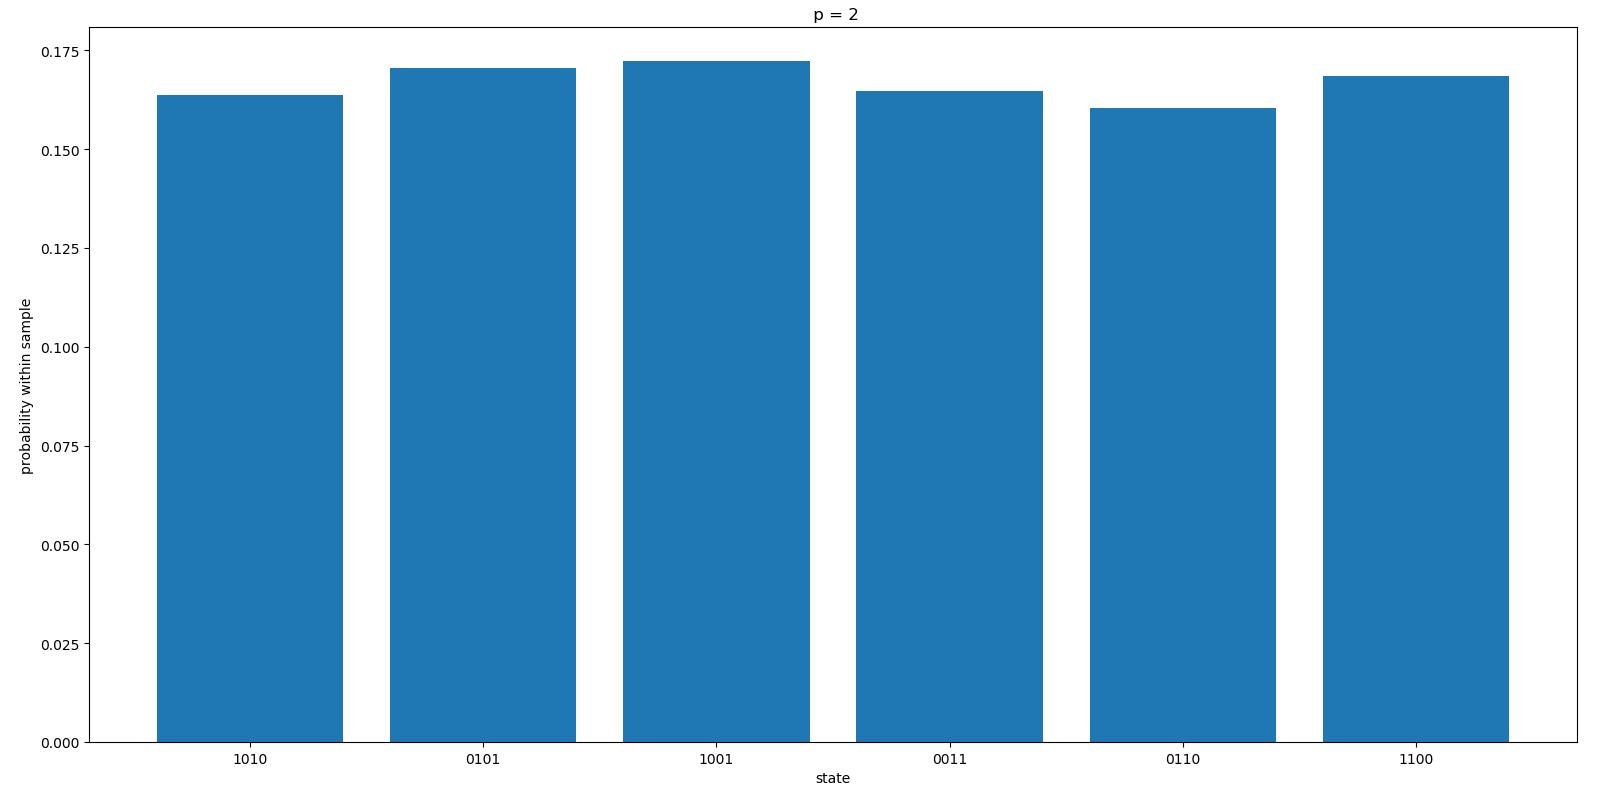
\includegraphics[scale=0.3,left]{figures/regular(3,4)-p2.png}
\end{figure}
\end{frame}

% 3-regular, 6 nodes
\begin{frame}{3-regular graphs - 6 nodes}
\begin{figure}
	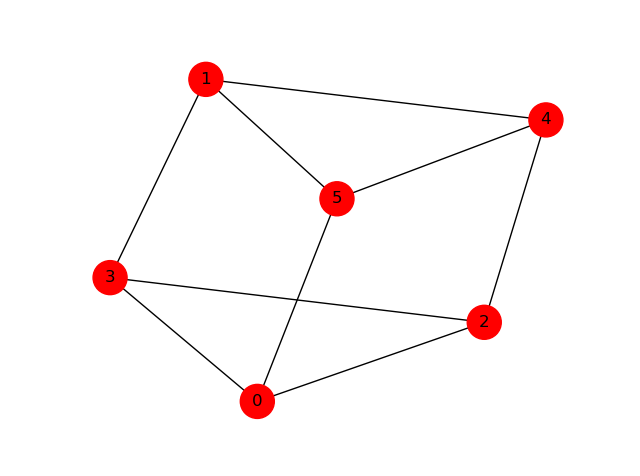
\includegraphics[scale=0.6]{figures/regular(3,6)-graph.png}
	\caption*{Optimal cuts are the ones with one neighbour pair and their opposite, for example $\{2,3,5\}$. You can form 6 of those. \textbf{labelling wrong in figure?}}
\end{figure}
\end{frame}

\begin{frame}{(3,6)-regular, $p = 1$}
\begin{figure}
\centering
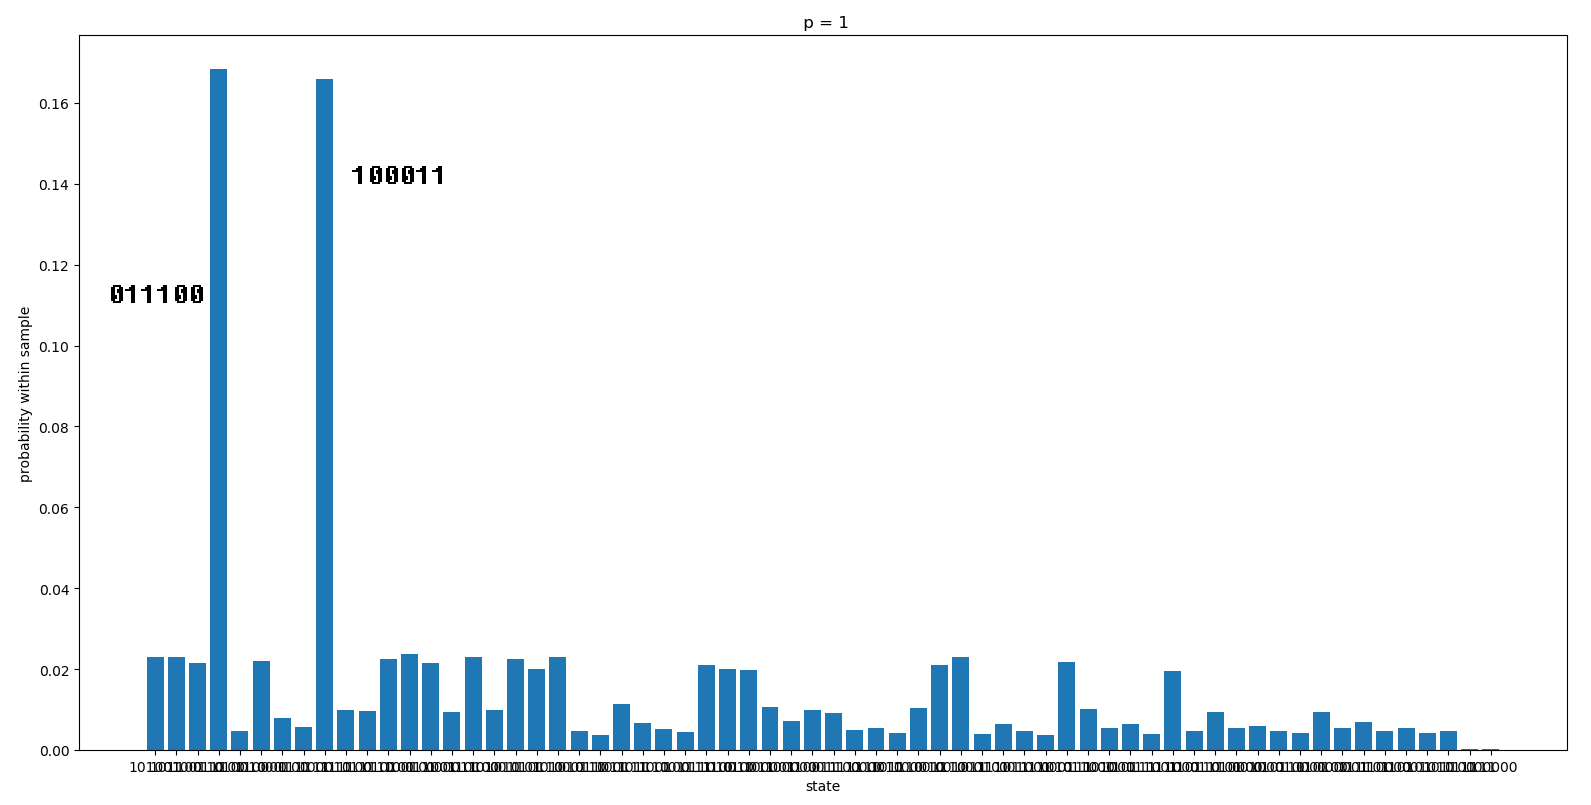
\includegraphics[scale=0.3,left]{figures/regular(3,6)-p1.png}
\end{figure}
\end{frame}

\begin{frame}{(3,6)-regular, $p = 2$}
\begin{figure}
\centering
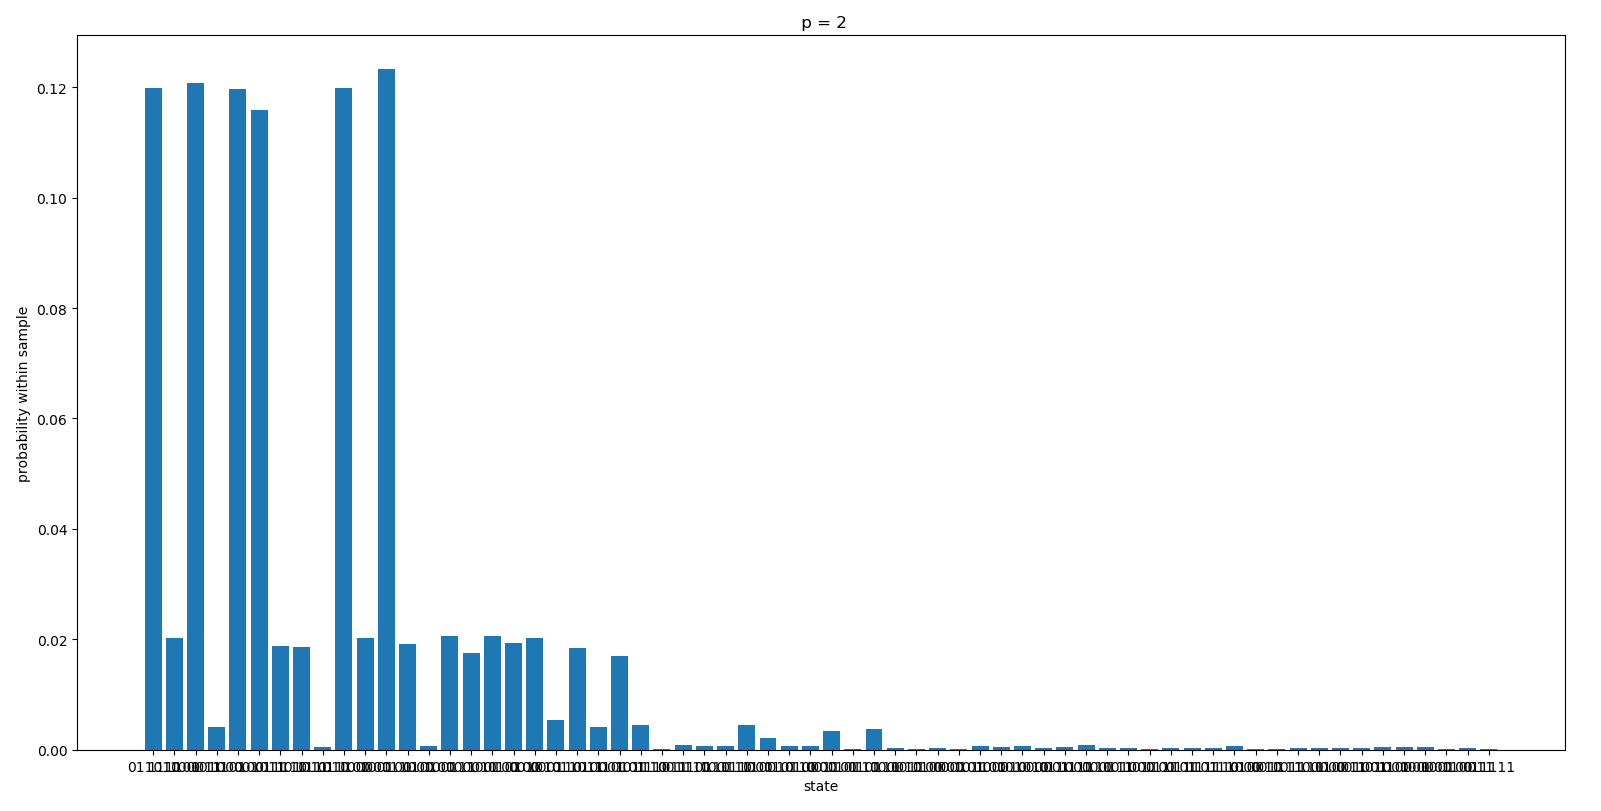
\includegraphics[scale=0.3,left]{figures/regular(3,6)-p2.png}
\end{figure}
\end{frame}

\section{Approximation ratio on 3-regular graphs}
\begin{frame}{Approximation ratio on 3-regular graphs}
	In the original QAOA paper from 2014 it was proven that for $p=1$, QAOA has a (worst case) approximation ratio $\rho = 0.6924$ meaning
	\begin{equation}
	\max_{\mathbf{z}} C(\mathbf{z}) \geq C(\mathbf{z}^*) \geq \rho \max_{\mathbf{z}} C(\mathbf{z})
	\end{equation}
	meaning that the optimal circuit produced a distribution of states with a Hamiltonian expectation value of 0.6924 of the true maximum cut for 3-regular graphs.
\end{frame}

\begin{frame}{Approximation ratio on 3-regular graphs}
For the  MaxCut problem there exists an approximate algorithm 1995 by Goemans and Williamson. This algorithm has an approximation ratio of  $\rho \approx 0.87856$. This approximation ratio is believed to optimal so it is not expected to see an improvement by using a quantum algorithm. (I don't know exactly why?)
\end{frame}


\section{Adiabatic Theorem}
\begin{frame}{Larger $p$ and the Adiabatic theorem}
	Using the adiabatic theorem it can be proven that
	\begin{equation}
		\lim_{p\to \infty} M_{p} = \max_{z} C(z)
	\end{equation}
	where
	\begin{equation}
	M_{p} = \max_{\vec{\gamma},\vec{\beta}} F_p(\vec{\gamma},\vec{\beta})
	\end{equation}
	However, the scaling of the algorithm with $p$ is (possibly?) not efficient. This depends on your method of determining these angles and I am not sure yet how VQE scales. %Should I look into quantum algorithmic complexity?
\end{frame}

\section{Further investigation}
\begin{frame}{Further investigation}
	\begin{itemize}
		\item larger graphs
		\item regular graphs analytically
		\item scaling of $p$
		\item other optimization methods such as pyswarm
		\item compare with Goemans-Williamson
		\item compare with Qiskit
		\item run on actual quantum chips
		\item use qaoa on other problems $\implies$ other cost Hamiltonian
		\item use other mixers
	\end{itemize}
\end{frame}

\end{document}
